\documentclass[fleqn,letterpaper,12pt,printwatermark=false]{memoir}
% memoir commands to define the text block geometry
\setulmarginsandblock{0.5in}{*}{*}
\setlrmarginsandblock{0.5in}{*}{*}
% put "extra" vertical space at the bottom of a page
\raggedbottom 

\usepackage{amsmath}
\usepackage{etoolbox} % for \ifblank etc
\usepackage{xparse} % for NewDocumentCommand et al.
\usepackage{enumitem}
\usepackage{transparent} % for \transparent, which I use in the watermark
\usepackage[slantedGreek]{mathpazo} \usepackage{helvet} % use Palatino et al.
\usepackage{booktabs} % prettier tables

\usepackage[]{xwatermark}
\newwatermark*[
    allpages,
    color=red!30,angle=45,
    scale=4,
    xpos=-10, ypos=0
]{%
    \transparent{0.4}dhasan example%
}

\usepackage{dashundergaps} % for \gap
\dashundergapssetup{
    teacher-mode=true, % set to true to show answers 
    gap-format=underline,
    teacher-gap-format=underline,
    gap-font={\sffamily},
    gap-numbers=true,
    gap-widen=true,
    gap-extend-percent=150, % note: making this too big might create errors
    gap-number-format=\,\textsuperscript{\normalfont(\thegapnumber)},
}

\usepackage{tcolorbox}
\tcbuselibrary{skins}
\tcbuselibrary{raster}

\usepackage{graphicx}
\graphicspath{ {../images/} }
\begin{document}

\newcommand{\myClassName}{Pre-AP Algebra 2}
\newcommand{\myUnitNumber}{1}
\newcommand{\myUnitTitle}{Introduction to Functions}
\newcommand{\myLessonNumber}{8}
\newcommand{\myLessonTitle}{Composing Functions}


\copypagestyle{myPagestyle}{empty}


\newcommand{\myFooterSize}{\footnotesize}
\makeoddfoot{myPagestyle}{{}}{\myFooterSize{\thepage{}~of~\pageref*{xwmlastpage}}}{\myFooterSize\thetitle}
\makeevenfoot{myPagestyle}{{}}{\myFooterSize{\thepage{}~of~\pageref*{xwmlastpage}}}{\myFooterSize\thetitle}

%
% A command to change the appearance of the cognitive verb 
% in the objectives.
%
\newcommand{\myCognitiveVerb}[1]{\textcolor{blue}{\textbf{#1}}}

%
% Terminology explanation:
%
% "unit" refers to the Algebra 2 unit being taught.
% "section" refers to the section within the unit being taught.
% "heading" refers to the headings in this document (Objectives, Example, ...)
%
\NewDocumentCommand{\myUnitSectionNumberFont}{}{\sffamily\bfseries\HUGE}
\NewDocumentCommand{\myUnitNameFont}{}{\sffamily\large}
\NewDocumentCommand{\mySectionNameFont}{}{\sffamily\bfseries\huge}
\NewDocumentCommand{\myHeadingFont}{}{\sffamily\bfseries\Large}


%
% #1 is the fill-in text
%
\NewDocumentCommand{\myFillInBlank}{m}{%
    \,%
    \gap[u]{#1}%
    \,%
}


% Definition for the LESSON HEADER + OBJECTIVES
%
% #1 : optional unit name
% #2 : optional unit/section number
% #3 : mandatory title
%
\NewDocumentEnvironment{myNotesHeader}{oom}{
    \title{#3}
    \begin{flushleft}
        \IfValueT{#2}{{\myUnitSectionNumberFont#2}}
        \hfill\;\;
        \begin{minipage}[b]{0.75\textwidth}
            \begin{flushright}
                \IfValueT{#1}{
                    {\myUnitNameFont#1}\\ \vspace{0.75em}
                }
                {\mySectionNameFont#3}
            \end{flushright}
        \end{minipage}
        \hrule
    \end{flushleft}
    \noindent{\myHeadingFont Objectives:}
    \begin{enumerate}[label=\arabic*)]
}{
    \end{enumerate}
}


% Definitions related to the VOCABULARY TABLE
%
\newenvironment{myVocabulary}{
    {\noindent{\myHeadingFont Vocabulary:}}\vspace{1em}

    \begin{tabular}{ll}
        \toprule
            \emph{word} & \emph{meaning} \\ 
        \midrule
}{
    \bottomrule
    \end{tabular}
    \vspace{1em}
}

\newcommand{\myVocabularyWord}[2]{%
{\textcolor{blue}{\textbf{#1}}} & #2 \\
}


% Definitions related to an INTRODUCTION
%
\newenvironment{myIntroduction}{
    {\noindent{\myHeadingFont Introduction:}}\vspace{1em}

    \setlength{\leftskip}{3cm}
}{
    \setlength{\leftskip}{0pt}
}


% Definition related to KEY CONCEPTS
%
% #1 : the key concept (which appears as a tcolorbox title)
%
\NewDocumentEnvironment{myKeyConcepts}{ O{Key Concepts:} }{
    \begin{tcolorbox}[
        title=#1, fonttitle=\myHeadingFont,
        coltitle=black, 
        colbacktitle=black!25!yellow, 
        colframe=black!50!yellow,
        colback=white!70!yellow,
        boxrule=2pt, 
        ]
}{
    \end{tcolorbox}
}


% Definition related to EXAMPLES
%
% #1 Optional example number 
% #2 A statement of the example problem.
% #3 How much empty vertical space to leave for the example box.
%
\NewDocumentCommand{\myExample}{omm}{%
    \begin{tcolorbox}[
        enhanced,
        sharp corners, 
        colback=white,
        boxrule=0pt,
        borderline={0.5pt}{0pt}{black,dashed},
        ]
        {\myHeadingFont Example\IfValueT{#1}{{ #1}}:}
        #2
        \tcblower
        \vspace{#3}
    \end{tcolorbox}
}

% Definitions related to PROBLEMS

% A counter to number the problems in the guided notes.
\newcounter{MyProblemCounter}
\setcounter{MyProblemCounter}{1}
\newcommand{\useMyProblemCounter}{\theMyProblemCounter\stepcounter{MyProblemCounter}}

% an environment for two adjacent problems
%
% #1 : directions for all the problems
% #2 : vertical height of the problem boxes
% #3 : details for problem 1
% #4 : details for problem 2
%
\newenvironment{myProblems2}[4]{%
    \noindent
    {\myHeadingFont Practice:}\hspace{0.5em}#1\nopagebreak%
    \begin{tcbraster}[%
        raster equal height,%
        raster columns=2,%
        raster column skip=0.5mm,%
        raster row skip=0.5mm,%
        raster every box/.style={%
            enhanced,%
            sharp corners,%
            colback=white,%
            coltitle=black, colbacktitle=black!10!white,%
            boxrule=0pt, borderline={0.5pt}{0pt}{black},%
            title={\texttt\useMyProblemCounter},%
            },%
        ]%
        \begin{tcolorbox}[attach boxed title to top left]
            #3
            \tcblower\vspace{#2}
        \end{tcolorbox}
        \begin{tcolorbox}[attach boxed title to top right]
            #4
            \tcblower
        \end{tcolorbox}%
}{%
    \end{tcbraster}
}

% an environment for 4 adjacent problems
%
% #1 : directions for all the problems
% #2 : vertical height of the problem boxes
% #3 : details for problem 1
% #4 : details for problem 2
% #5 : details for problem 3
% #6 : details for problem 4
%
\newenvironment{myProblems4}[6]{%
    \noindent
    \textbf{\myHeadingFont Practice:}\hspace{0.5em}#1\nopagebreak%
    \begin{tcbraster}[%
        raster equal height,%
        raster columns=2,%
        raster column skip=0.5mm,%
        raster row skip=0.5mm,%
        raster every box/.style={%
            enhanced,%
            sharp corners,%
            colback=white,%
            coltitle=black, colbacktitle=black!10!white,%
            boxrule=0pt, borderline={0.5pt}{0pt}{black},%
            title={\texttt\useMyProblemCounter},%
            },%
        ]%
        \begin{tcolorbox}[attach boxed title to top left]
            #3
            \tcblower\vspace{#2}
        \end{tcolorbox}
        \begin{tcolorbox}[attach boxed title to top right]
            #4
            \tcblower
        \end{tcolorbox}%
        \begin{tcolorbox}[attach boxed title to bottom left]
            #5
            \tcblower
        \end{tcolorbox}%
        \begin{tcolorbox}[attach boxed title to bottom right]
            #6
            \tcblower
        \end{tcolorbox}%
}{%
    \end{tcbraster}
}
\pagestyle{myPagestyle}

\checkandfixthelayout
\setlist{labelindent=\parindent,leftmargin=*,itemsep=0.025em,label=$\circ$}

% ---------------------HEADER------------------------------
\begin{myNotesHeader}
    \item \myCognitiveVerb{evaluate} a composite fuction with a number
    \item \myCognitiveVerb{compose} two functions
\end{myNotesHeader}

\begin{myVocabulary}
    \myVocabularyWord{compose}
        {
            construct something from smaller pieces
        }
        \myVocabularyWord{composing functions}
        {
            construct a function from smaller functions
        }
        \myVocabularyWord{composite function}
        {
            a function composed from smaller functions
        }
\end{myVocabulary}

% ---------------------LESSON 1------------------------------
\begin{myLesson}[Functions as Meat Grinders]
    A function can be thought of as a \emph{meat grinder}.\footnote{
        My apologies to vegetarians and vegans.
    }
    You put chunks of beef into a meat grinder (the \emph{input}),
    and ground hamburger comes out (the \emph{output}). 

    \begin{center}
    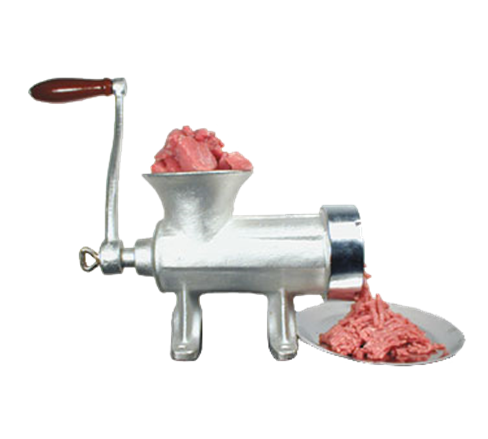
\includegraphics[width=1.5in]{meat-grinder.png} 
    \end{center}

    \begin{center}
    \(
        \text{chunks of beef}
        \Longrightarrow
        \text{meat-grinder-function}
        \Longrightarrow
        \text{ground hamburger}
    \)
    \end{center}

    Similarly,
    in math a function has \emph{inputs} and \emph{outputs}.
    We usually use $x$ for the inputs and $y$ as the outputs.
    You put $x$'s into a function, $f(x)$,
    and $y$'s come out.
    Think of the $x$'s as the chunks of beef
    and the $y$'s as the ground hamburger.
    \begin{center}
    \(
        x
        \Longrightarrow
        f
        \Longrightarrow
        y
    \)
    \end{center}

    You could ``daisy chain'' two meat grinders---when 
    you take the output of one function and put it into
    another one.
    The two griders act as a  
    \emph{single, bigger meat grinder} which takes chunks of beef
    as an input and creates 
    {\bfseries\itshape ultra-ground beef} as an output.

    \begin{center}
        \fbox{
            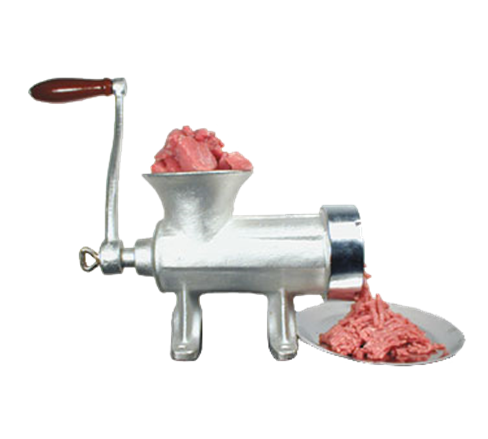
\includegraphics[width=1.5in]{meat-grinder.png} 
            \hspace{0.5in}
            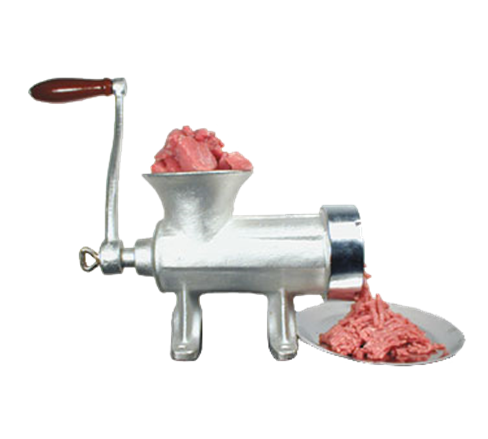
\includegraphics[width=1.5in]{meat-grinder.png} 
        }
    \end{center}
    To emphasize that the two grinders work together, 
    we could draw it like this
    \begin{center}
        \fbox{
            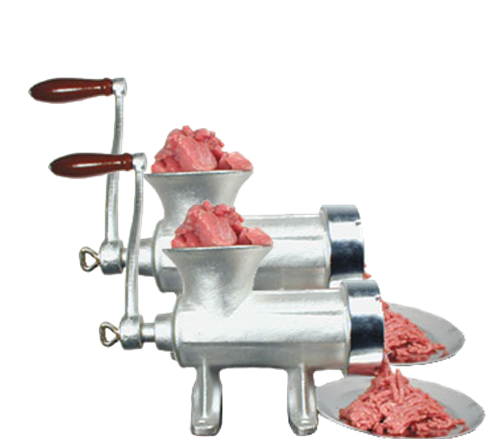
\includegraphics[width=1.5in]{composite-meat-grinder.png} 
        }
    \end{center}
    This is called ``composing''. 
    We have composed two meat grinders
    into a single, bigger grinder in the box that is called 
    a ``composite grinder''.

    In math, when you do this to functions,
    you are ``composing'' the two functions
    into \emph{single, bigger functions}.
    We call these ``composite functions''.

    \begin{center}
    \vspace{1em}
    \(
        x
        \Longrightarrow
    \)
    \fbox{
        \(
            f
            \Longrightarrow
            g
        \)
    }
    \(
        \Longrightarrow
        y
    \)
    \vspace{1em}
    \end{center}
    That thing in the box is a composite function,
    which is what you will learn about next.
\end{myLesson}

\begin{myLesson}[][1]
    Consider the following functions.
    \begin{align*}
        f(x) &= 2x + 3 \\
        g(x) &= -x^2 + 5
    \end{align*}
    You already know how to evaluate them at (say) $x=1$:
    \begin{align*}
        f(1) &= 2(1) + 3   = 2+3    = 5\\
        g(1) &= -(1)^2 + 5 = -1 + 5 = 4
    \end{align*}
    When we \emph{compose} functions, 
    we evaluate one of them and take the {\bfseries\itshape output} and pass it 
    into the other one.

    The math notation for function composition looks like this:
    $f \circ g$,
    which you pronounce as ``$f$ compose with $g$''. 
    But be careful.
    The order of the functions matters.
    \begin{myLessonBox}[3in]
        $(f \circ g)$ 
        and
        $(g \circ f)$ 
        are not the same.
    \end{myLessonBox}
\end{myLesson}

% ---------------------CONCEPT 1------------------------------
\begin{myKeyConcepts}[To evaluate a composite function at a number\dots]
    Follow these steps:
    \setlist{labelindent=\parindent,}
    \begin{enumerate}
        \item {\bfseries\itshape Pass} the number input to the nearest function to the left.
        \item {\bfseries\itshape Evaluate} that nearest function. (You will get a number.)
        \item {\bfseries\itshape Pass} that value to the next function to the left. 
        \item {\bfseries\itshape Evaluate} the that next function. (You will get a number.)
    \end{enumerate}
    When the functions are $f$ and $g$ and the number is $2$,
    \begin{align*}
        (f \circ g)(2) &= f(g(2)) \\
        (g \circ f)(2) &= g(f(2))
    \end{align*}
\end{myKeyConcepts}

\myExample{
    Evaluate the composite functions 
    $(f \circ g)(2)$ and $(g \circ f)(2)$ where
    \begin{align*}
        f(x) &= x + 2 \\
        g(x) &= 3x - 4
    \end{align*}
}{3in}

% \myExample{
%     Evaluate the composite functions $(f \circ g)(2)$ and $(g \circ f)(2)$ where
%     \begin{align*}
%         f(x) &= 2x + 3 \\
%         g(x) &= -x^2 + 5
%     \end{align*}    
% }{3in}

\myExample{
    Evaluate $(v \circ w)(3)$ and $(w \circ v)(3)$ where
    \begin{align*}
        v(t) &= t + 1 \\
        w(t) &= t^2 + 2t + 3
    \end{align*}    
}{3.5in}

You can compose a function with itself.

\myExample{
    Evaluate $(w \circ w)(-2)$ where
    \begin{align*}
        w(z) &= z^2 - z
    \end{align*}    
}{3.7in}

% ---------------------LESSON 2------------------------------
\begin{myLesson}[][2]
    What would you do with
    $(f \circ g)(x)$
    where the input is a variable instead of a number?
    It turns out that the ideas are the same as what you just learned.
\end{myLesson}

% ---------------------CONCEPT 2------------------------------
\begin{myKeyConcepts}[To compose two functions\dots]
    Follow these steps:
    \setlist{labelindent=\parindent,}
    \begin{enumerate}
        \item {\bfseries\itshape Pass} the variable input to the nearest function to the left.
        \item {\bfseries\itshape Evaluate} that nearest function. (You will get an algebraic expression.)
        \item {\bfseries\itshape Pass} that expression to the next function to the left. 
        \item {\bfseries\itshape Evaluate} the that next function. (You will get an algebraic expression.)
    \end{enumerate}
    When the functions are $f$ and $g$ and the variable is $x$,
    \begin{align*}
        (f \circ g)(2) &= f(g(x)) \\
        (g \circ f)(2) &= g(f(x))
    \end{align*}
\end{myKeyConcepts}

\myExample{
    Evaluate the composite functions 
    $(f \circ g)(x)$ and $(g \circ f)(x)$ where
    \begin{align*}
        f(x) &= x + 2 \\
        g(x) &= 3x - 4
    \end{align*}
}{4in}

% \myExample{
%     Evaluate the composite functions $(f \circ g)(x)$ and $(g \circ f)(x)$ where
%     \begin{align*}
%         f(x) &= 2x + 3 \\
%         g(x) &= -x^2 + 5
%     \end{align*}    
% }{3in}

\myExample{
    Evaluate $(v \circ w)(t)$ and $(w \circ v)(t)$ where
    \begin{align*}
        u(t) &= t + 1 \\
        v(t) &= t^2 + 2t + 3
    \end{align*}    
}{3.75in}

\myExample{
    Evaluate $(w \circ w)(z)$ where
    \begin{align*}
        w(z) &= z^2 - z
    \end{align*}
}{3.75in}

% \begin{myProblems2}%
%     {Factor the following monomials into prime factors.}%
%     {2in}%
%     %
%     {\( 32x^2 \)}
%     {\( 8 x^3y^2z \)}
% \end{myProblems2}
  


\end{document}